%%  'printversion' pro sazbu verze pro tisk (nebarevné logo a odkazy,
%%  odkazy s uvedením adresy za odkazem, ne odkazy do rejstříku),
%%  jinak verze pro prohlížeč

%%  'biblatex' pro zapnutí podpory pro sazbu bibliografie pomocí
%%  BibLaTeXu, jinak je výchozí sazba v prostředí thebibliography

%%  'language=jazyk' pro jazyk práce, jazyky english pro anglický,
%%  slovak pro slovenský, jinak je výchozí czech pro český

%%  'font=sans' pro bezpatkový font (Iwona Light), jinak je výchozí
%%  serif pro patkový (Latin Modern)

%%  'figures, tables, theorems a sourcecodes' pro sazbu seznamu
%%  obrázků, tabulek, vět a zdrojových kódů, jinak při =false se
%%  nesází (u theorems a sourcecodes výchozí)

\documentclass[
%  printversion,
 % biblatex,
  language=english,
%  font=sans,
  figures=false,
%  tables=false,
  sourcecodes,
%  glossaries,
  index
]{kidiplom}

%% Informace pro úvodní strany. V jazyku práce (pokud není v komentáři
%% uvedeno česky) a anglicky. Uveďte všechny, u kterých není v
%% komentáři uvedeno, že jsou volitelné. Při neuvedení se použijí
%% výchozí texty. Text pro jiný než nastavený jazyk práce (nepovinným
%% parametrem language makra \documentclass, výchozí český) se zadává
%% použitím makra s uvedením jazyka jako nepovinného parametru.

%% Název práce, česky a anglicky. Měl by se vysázet na jeden řádek.
\title[czech]{Vytvoření komplexní aplikace pro iOS pomocí SwiftUI a Swift Backend Development}
\title[english]{Building a comprehensive iOS application with SwiftUI and Swift Backend Development}

%% Jméno autora práce. Makro nemá nepovinný parametr pro uvedení
%% jazyka.
\author{Maksym Kupchenko}

%% Jméno vedoucího práce (včetně titulů). Makro nemá nepovinný
%% parametr pro uvedení jazyka.
\supervisor{Mgr. Roman Vyjídáček, Ph.D.}

%% Volitelný rok odevzdání práce. Výchozí je aktuální (kalendářní)
%% rok. Makro nemá nepovinný parametr pro uvedení jazyka.
\yearofsubmit{2024}

%% Anotace práce, včetně anglické (obvykle překlad z jazyka
%% práce). Jeden odstavec!
\annotation[czech]{Závěrečná práce se zabývá vývojem serveru Vapor s PostgreSQL a mobilní aplikací SwiftUI pro iOS. Zahrnuje vývoj Swift na straně serveru, ověřování, ověřování dat a zpracování chyb. Práce hodnotí výkon, použitelnost a bezpečnost. Přispívá ke znalostem o Swift na straně serveru a ukazuje potenciál Vapor a SwiftUI pro škálovatelná řešení aplikací pro iOS.}

\annotation[english]{Bachelor thesis explores the development of a Vapor server with PostgreSQL and a SwiftUI iOS application. It covers server-side Swift development, authentication, data validation, and error handling. The work evaluates performance, usability, and security. It contributes to knowledge on server-side Swift, showcasing the potential of Vapor and SwiftUI for scalable iOS app solutions.}

%% Klíčová slova práce, včetně anglických. Oddělená (obvykle) středníkem.
\keywords[czech]{Mobilní aplikace;Swift; Vapor; SwiftUI; iOS; PostgreSQL}
\keywords[english]{Mobile application; Swift; Vapor; SwiftUI; iOS; PostgreSQL}

%% Volitelná specifikace příloh textu práce, i anglicky. Výchozí je
%% 'elektronická data v systému katedry informatiky / electronic data
%% in system of department of computer science'.
%\supplements{nejlepší software všech dob}
%\supplements[english]{the best software of all times}

%% Volitelné poděkování. Stručné! Výchozí je prázdné. Makro nemá
%% nepovinný parametr pro uvedení jazyka.

%% Cesta k souboru s bibliografií pro její sazbu pomocí BibLaTeXu
%% (zvolenou nepovinným parametrem biblatex makra
%% \documentclass). Použijte pouze při této sazbě, ne při (výchozí)
%% sazbě v prostředí thebibliography.
%\bibliography{bibliografie.bib}

%% Další dodatečné styly (balíky) potřebné pro sazbu vlastního textu
%% práce.
\usepackage{lipsum}
\usepackage{longtable}
\usepackage{graphicx}
\graphicspath{ {text/} }

\begin{document}
%% Sazba úvodních stran -- titulní, s bibliografickými údaji, s
%% anotací a klíčovými slovy, s poděkováním a prohlášením, s obsahem a
%% se seznamy obrázků, tabulek, vět a zdrojových kódů (pokud jejich
%% sazba není vypnutá).
\maketitle

%% Vlastní text závěrečné práce. Pro povinné závěry, před přílohami,
%% použijte prostředí kiconclusions. Povinná je i příloha s obsahem
%% elektronických dat.

%% -------------------------------------------------------------------

\newcommand{\BibLaTeX}{\textsc{Bib}\LaTeX}

\section{Introduction}

Today's trend is leaning towards mobile-first solutions, as mobile platforms offer faster and more intuitive user experiences. At present, there exist loads of web-based and multi-platform applications for task management, catering to the needs of users. However, there is a noticeable absence of a native mobile application.

My motivation arises from the need to streamline task management processes in school and provide users with a more convenient means of organising their tasks effectively.

In this bachelor thesis, I aim to design and implement a server-side and an iOS application focused on task management, named "StudentChrono". This application will empower users to easily create, update, track and solve their tasks, and categorise them based on priority or deadline. "StudentChrono" will serve as a comprehensive tool for users to manage their tasks efficiently.

In the first chapter, I look into the theoretical basis and technologies needed to create the iOS platform's application development, architecture, and programming paradigm in addition to other patterns utilised in server-side and mobile development. I analyse services that are appropriate for integration and lay down the specifications for the application in the second chapter. I use the technologies and concepts from earlier chapters to explain the application's software engineering process, which includes architecture, design, implementation, and testing.

\section{Thesis Goal}
The primary goal of this bachelor thesis is to implement StudentChrono iOS mobile application for students and teachers integrated with server-side application, which is also part of this bachelor thesis. Teachers can manage theirt students, create tasks and evaluate them, provide deadline, priorities, detailed information and files needed for task elaboration. Students can view detailed information about tasks, solve them and send feedback to a teacher. In addition, every user is able to delete account, manage their personal account and provide feedback for developers.

In the research part, the aim is to summarise specifics of iOS development and other technologies related to mobile application development. The second goal is to investigate server-side development with Swift programming language.

In practical part objectives are designing application requirements and user interface, choose software architecture, implement the server and the mobile application, describe release process.

\section{Technologies and Solutions}

In this chapter I describe the theoretical background, possible solutions and technologies used later in this work - specifics of development for iOS platform, server-side development with Swift programming language, REST API and it's usage in modern applications' development, authorisation and authentication protocols.

\subsection{Swift programming language}
Swift is a strongly typed, compiled modern language supporting modern trends. It was first introduced in 2014 at the Apple Worldwide Developers Conference (WWDC). Apple Inc. developed Swift as a modern language to replace Objective-C on their platforms. According to the book by John Hoffman \cite{bib2}, it offers concepts such as type inference, genericity, closure syntax, optional types and many others. Thanks to these concepts, Swift became one of the fastest growing languages shortly after its introduction. The fact that in 2015 Apple made the source code available to the general public also contributed to this, making the entire Swift an open source project. Another major influence was that even though Swift was designed for Apple platforms, its code can be compiled with limitations on platforms other than Linux or Windows. However, the limitations of compilation on other platforms are rapidly decreasing, and the gradually increasing support of Swift by the Ubuntu operating system allows the development of server applications in the Swift language as well. According to the official site \cite{bib3}, the Swift language is intuitive and designed for application security.

\subsubsection{Swift basics}
Swift is derived from languages inspired by C. Although it was designed as a replacement for Objective-C, it can be combined with it. In addition, a combination with C++ and C languages is also possible thanks to its LLVM compiler. In order to free up operational memory, Swift uses the concept of deterministic reference counting to work with memory. Thanks to this concept, there is no need for a garbage collector searching for unreachable memory. The number of references is incremented when creating strongly referenced variables. This count is decremented when the object is dereferenced. Whenever the reference count is reduced to zero, the memory is automatically freed.

Swift also gets rid of dangerous concepts such as uninitialized variables. Furthermore, it helps prevent incorrect work with variables that can acquire the value nil (representing NULL). The type of such variables is marked with a ? (question mark) and represent the so-called optional value. The Swift language offers special constructs for working with an optional type that force programmers to explicitly handle the case when a variable takes on the value nil. One of these constructions is also ! (exclamation mark). Its task is to access the value of an optional variable. However, its use is dangerous, because if there is no value in the variable, or if this value is nil, the entire application will crash. Source code 1 clearly shows how the optional type behaves and how it is possible to work with it.

\begin{kicode}{Swift}{code1}{Demonstration of work with variable of type optional Int}
// Definition of constant with optional type Int and value 2
let optionalValue: Int? = 2 // type Int? == Optional<Int>
Error optional value must be unwrapped
let optionalValueError = 1 + optionalValue
// If optionalValue is nil whole application shuts down
let onePlusOptionalValueBreak = 1 + optionalValue! // force unwrapping
// nil coalescing operator ??
let onePlusOptionalOrZero = 1 + (optionalValue ?? 0)
// proper way to unwrapp value
if let optionalValue {
// Work with optional value
} else {
// Handle nil value
}
\end{kicode}

\subsubsection{Enumeration type Enum}
The difference between the commonly supported enumeration types and the Enum type in Swift is that Swift supports value binding. This means that each instance of the enumeration can be assigned a value. Assigning values is possible in two ways. The first method determines the value type of all instances. Within the given type, it is then possible to assign a constant raw value to each case of enumeration.

The second option is the type of enumeration with associated values (associated values). It allows the programmer to define for each instance the type of value that can be stored in that enumeration instance. A declaration of this type is in Source code 2.

\begin{kicode}{Swift}{code2}{Enumeration with associated values}
// Declaration of Enum with associated values
enum EnumExample {
// Cases can have different types of associated values
	case first(String)
// Cases can have different number of parameters
	 case second(Int, String)
	 case third([Double])
}
\end{kicode}

\subsubsection{Protocols in Swift}
Swift also supports protocol programming. This is similar to the required override/overload of inheritance in objects. It is a concept in which there is a protocol, or a plan describing and requiring certain methods or properties. Then this plan can be adopted by structures, classes, or appointment types. Acceptance consists in implementing all protocol requirements.

\subsubsection{Data type structure and class}
In Swift, the structure is extended compared to other languages in such a way that it is possible to define methods in it, which makes it indistinguishable from a class at first glance. The difference is how they are handled within the RAM. The structure is sold by value. This means that when you pass a structure to a function, the entire instance of the structure is copied onto the stack. Unlike a structure, a class is sold by reference, which means that when sold to a function, only a reference to the location in memory where the class instance resides is copied.

\subsubsection{Closures}
Unnamed blocks of code that can be executed in a different part of the code in which they were defined are called closures in Swift. Swift differs from other programming languages that offer similar concepts in that closures save their context in addition to the given code. Swift offers great syntactic support for closures. It allows, for example, to write a closure for calling a function that receives this closure as the last parameter.

\subsection{Programming applications for iOS devices}
For mobile application programming, the programmer must realize that the application must always take care of something. This means that it must always be ready for various events, such as minimizing the application, either by the user or by incoming phone calls. Therefore, Apple precisely defines the states in which the application can be. Each of the states also defines what the application can and cannot do in this state. State indicates whether application windows are in the foreground, background, or transitioning to one of these states.

\subsubsection{Application life cycle}
As the application works and changes its state, the programmer must adjust its behavior to suit the current state. For example, if an application is in the background, it should not perform any activity. \ref{fig:image2} shows individual possible states that make up the life cycle of the application\cite{bib4}.

%\begin{figure}[t]
%\centering
%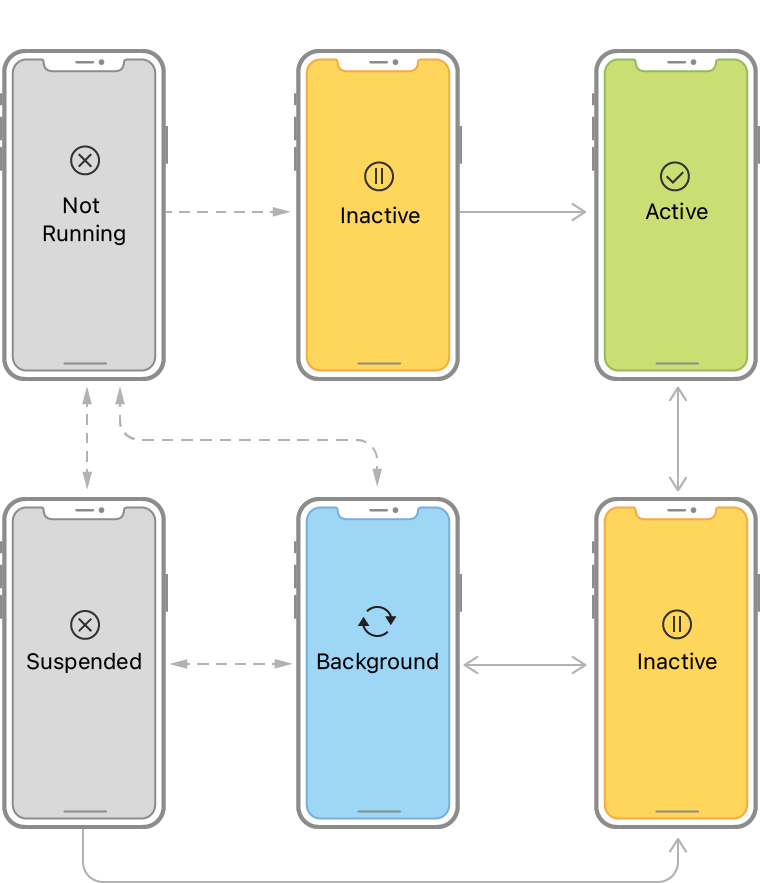
\includegraphics[width=8cm]{image2}
%\capition{Lifecyle of iOS application}
%\label{fig:image2}
%\end{figure}

The picture shows that the application does not work at the beginning. At startup, the main window is inactive and the application has time to load the necessary data. Due to the imprecise name of the state, it should be noted that the inactive application is actually still running in the foreground, but is not receiving any events. After loading the data, the application is presented to the user and events are sent to it. From this state, however, it can go into the background at any time, but it must go through the inactive state again. In the background, the application is then expected not to work or, with certain exceptions, to work only minimally. Another possible state is suspend, which the application enters when its code cannot be executed.

\subsubsection{Directly supported application architectures}
Apple Inc. directly supports the two architectures Model-View-Controller (MVC) and Model-View-ViewModel (MVVM) within Swift. In general, it is about dividing the system into three parts. The first is a framework that takes care of data storage and transformation. The second part is something that displays the data. In addition, the second part takes care of individual user inputs to the system. The last part is a kind of bridge between the first two parts.

MVC is one of the most widely used types of system architectures, so it has been supported in Swift since the beginning. This support is provided by the UIKit library for iOS. However, in this architecture, programmers often created a controller that was too comprehensive and often disrupted the correct division of the application into modules. But in 2019 came the SwiftUI library, which brought direct support for MVVM. 
The difference is that there is no Controller. In this architecture, the user interface is described as the state of the application. Displayed windows are composed of instances of a structure that implements the View protocol. These structures create views. In order for the window to be dynamic, and therefore to be redrawable based on some event, we can give special attributes to individual views. These attributes use two-way binding (Binding) with the ViewModel or directly with the Model. Then we understand the state precisely as the sum of the values of the bound attributes. This state is always stored in the ViewModel object, which takes care of displaying windows and their views. To redraw the window, the state of the application must be changed, that is, at least one attribute linked to a view must be changed. It is necessary to point out that the entire window is not always redrawn, but only its views to which the changed states are linked.

\subsubsection{SwiftUI Framework}
The SwiftUI framework represents a protocol known as a view, which must be adapted by the structure in order to be displayed. The protocol requires the definition of the point attribute, whose value also implements the View protocol. Source code 3 shows the creation of a simple view that contains the text "Hello, World!" and globe icon above it.

\begin{kicode}{Swift}{} {HelloWorldView.swift}
struct HelloWorldView: View {
    var body: some View {
        VStack {
            Image(systemName: "globe")
                .font(.system(size: 100))
                
            Text("Hello World!")
                .font(.title)
                .padding(.bottom)
        }
        .padding()
    }
}
\end{kicode}

\subsubsection{Handling view state}
Dynamics will be ensured by adding attributes that must be wrapped with a property wrapper (property wrapper, in the following text only the term wrapper is used) of a special type. A change in the wrapper values will then be propagated to the ViewModel, guaranteeing a redraw of the window. In his article [6], Paul Hudson explains the individual ways of tracking attribute changes.

The most important wrapper is \texttt{@State}, which can wrap attributes of simple data types and structures. Referenced types are observed using the @ObservedObject wrapper, which must implement the \texttt{ObservableOject} protocol. There is a \texttt{@Published} wrapper for marking tracked attributes in the referenced type. Referenced types can also be observed using the \texttt{@StateObject} wrapper, in which the application is responsible for the life cycle and not the user directly, as is the case with \texttt{@ObservedObject}. Another wrapper is \texttt{@EnviromentObject}, which allows you to get objects implementing the ObservableObject protocol that were created by views at a hierarchically higher level. Thanks to this, we do not have to sell these objects with arguments through several calls to views, which improves the overall readability of the code.

\subsubsection{Working with Views}
SwiftUI provides three basic window layout constructs: HStack, VStack, and ZStack. They are used to store views next to each other based on a specified axis. HStack places views next to each other (from left to right), VStack places them below each other (from top to bottom), and ZStack over them (from back to front).

Instead of the \texttt{Text} structure, we can insert points of other more complex structures into the body of the variable and thus create more complex windows and views. A \texttt{TextField} window is used to allow users to enter text. Using a parameter of type \texttt{Binding<String>}, this window can store input from the user in the variable provided by the parameter. A button represented by the Button structure is prepared for simple predefined user input. This structure requires two closures. The first defines what should happen when the button is pressed - the action, and the second defines the content of the button.

Views can be formatted and their final appearance can be changed. For example, the \texttt{Text} structure can be formatted with methods that change the appearance of the text. Such a method is, for example, the \texttt{font} method changing the font size or \texttt{.foregroundColor(Color)} changing the font color. FontWeight is used for thick font. The background color is changed using the background method. Changing the size of the view is possible with the \texttt{.frame} method.

\subsection{Server Application}
A server application has the task of mediating resources to one or, more often, to several users. While among the types of computer network structures it is possible to find, for example, a client-server structure, which indicates the work of a server application. So it is a structure in which there is one main device (server), which is connected to the network and has some resources available. There are also other devices connected to the network that want to access the server's resources. These devices are referred to as client stations or clients. The server application waits for requests from clients. Server requirements vary based on what clients require. Requests can be sent, for example, using the HTTP protocol.

\subsubsection{HTTP Protocol}
The abbreviation HTTP comes from the English name of the protocol (Hypertext Transfer Protocol or in Slovakian Hypertext Transfer Protocol) used on the worldwide network (World Wide Web, abbreviated WWW). It works on the application layer described by the open systems interconnection model (the abbreviation OSI from the English translation The Open Systems Interconnection is used)\cite{bib1}. The protocol works on the transport protocol of controlled transmission (known as the abbreviation TCP from the English term The Transmission Control Protocol).

Different types of HTTP requests have different semantics, but they may not be detailed enough for more complex servers. Therefore, servers tend to cluster work on some data. These clusters of data activities are then accessed using a uniform resource identifier (Uniform Resource Identifier or the more commonly used abbreviation URI), which is part of the URL in the HTTP request. The HTTP protocol uses nine types of requests, which are named as methods. The most used, and thus the most frequently supported, methods are GET, POST, PUT and DELETE. GET is a method used to get some data. The purpose of the POST method is to sell data to the server. PUT is used to replace some data. The DELETE request is intended to delete a document.
Each request must have a main header. Additional headers and their values are listed in the main header. The headers are, for example, the length of the body content (Content-length) or the authorized access header (Authorization), used for sending authorization code. The header can be followed by a body in which encoded data can be found.

\subsubsection{Programming of server applications}
When programming a server application, it is necessary to configure the server first. This configuration consists in creating and setting a kind of end point (the term socket is used in English), which connects the gateway (further on, only the English equivalent - port) of the device is used with the application. This configuration indicates to the operating system that the data sent to this device on this port is to be released to the application. The next step on the server side is to listen on that port. Listening means waiting until the operating system recognizes that a request has arrived for an application on a specified port. The operating system forwards the request to the application. The request should then be checked by the server and some work should be done. 

A frequently required practice is for the server application to always respond to the client with a message containing at least information on whether the request was processed correctly.
Although such a simple application will work correctly under certain circumstances, today's trend considers it incapable of normal functioning. If a new request arrives while the previous one is being processed, this request is ignored. To avoid dropping the right request due to load, requests can be stored in an array and processed sequentially. However, stored requests may not be processed quickly enough, so their time may run out. Therefore, processes and or threads are used. The application then has one main process that waits for requests in an infinite loop.

%\begin{figure}[t]
%\centering
%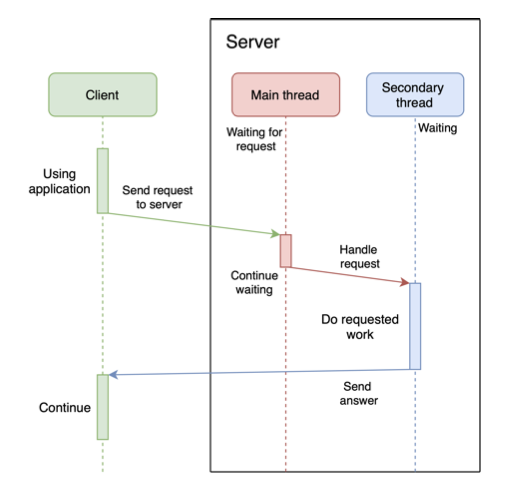
\includegraphics[width=8cm]{image1}
%\capition{Parallelisation of request handling}
%\label{fig:image1}
%\end{figure}

After receiving the request, the main process creates a new thread to handle the request and then continues to wait. The child thread processes the request, performs some operations, and sends the response back to the client. \ref{fig:image1} shows such a parallel reception of a request. The programmer then creates routes for individual supported request types and their possible variants or subsets. Paths have an identifier and some functionality. Thanks to the Identifier, it is possible to further divide the resources of the server application.

\subsection{Creating server applications using the Vapor framework}
The Vapor framework was created for creating server-side applications. It is a library with an expressive, protocol-oriented design focused on type safety. Vapor directly supports authentication using Basic or Bearer algorithms. It also supports working with database systems such as MySQL, PostgreSQL, SQLite and MongoDB. It allows you to create HTML templates, it also allows you to create client and server applications using HTTP and many other concepts.

\subsubsection{Vapor basics}
Like any server application, an application created in the Vapor framework waits in an infinite loop for queries. To do this, Vapor uses concurrency, which allows an endless loop processing input and output processes. In order to ensure the processing of as many requests arriving at a similar time as possible, it is possible to operate processes from several threads. Working with processes is based on the modern Async/Await principle, which simplifies work with multiple threads and asynchronous processes.
This principle works in such a way that an asynchronous process is executed on another thread, while an object representing the result of the asynchronous code obtained sometime in the future is created in the current thread. It is possible to call other functions above this object and thereby determine further processing of the asynchronous result.

\subsubsection{Request routing}
Routing in this context is creating paths. Identifiers (parts of the path separated by the / symbol) and assigned functionality are assigned to paths. In the Vapor library, this is done by registering individual paths. Registration consists of specifying the HTTP method, specifying the identifier and defining the function itself.
There is an instance of the Application class and thus represents a server application. Using its get method, a block of code is defined for handling HTTP messages of type GET with the path HelloWorld. The method allows creating more complex paths using a variable number of arguments. The last argument is the closure, whose parameter is an object of type Request. This object represents the received HTTP request. The closure must return a value of a type that implements the Content protocol, and thus the returned type can be represented as an HTTP response. The return value is then serialized and sent as a response to the HTTP request.

\subsubsection{Creating a database}
To access the database, it is necessary to set the configuration, this consists in entering login data, the name of the database and its location. Using this configuration, Vapor then takes care of connecting to the database. Vapor allows you to define and create database elements such as tables or initial data using migrations. The task of migration is to create or modify the table so that it appropriately represents the desired objects.Source code 4 shows the migration to create and revert the SomeModelTable table. In the statement, the name of the table is successively set, then two columns are created, and finally the entire table is created. Reverting database is also a part of every model migration.

\begin{kicode}{Swift}{}{Table creation using Vapor}
extension SomeModel {
    struct Migration: AsyncMigration {
        
        func prepare(on database: any Database) async throws {
            try await database.schema(schema)
                .id()
                .field(FieldKeys.name, .string, .required)
                .create()
        }
        
        func revert(on database: any Database) async throws {
            try await database.schema(schema)
                .delete()
        }
    }
}
\end{kicode}

\subsubsection{Model representation}
A model that represents a single record and its relationships is used to access the individual rows of the table. Source code 5 shows a simple model for a someModelTable that has two columns: id and name. SomeModel is a final class that adapts the Model and Content protocols. By defining the schema variable, the class determines to which table the instances of the class will belong. The id variable is wrapped with the \texttt{@ID} wrapper, which indicates the private key. The second variable is wrapped by the \texttt{Field} wrapper, which has the task of representing an ordinary table column. Structure \texttt{FieldKeys} contains column names.

\begin{kicode}{Swift}{}{Model representing in Vapor}
final class SomeModel: Model {
    
    static let schema: String = SchemaEnum.someModel.rawValue
    
    @ID
    var id: UUID?
    
    @Field(key: FieldKeys.name)
    var name: String
}
extension SomeModel {
    struct FieldKeys {
        static var name: FieldKey {"name"}
    }
}
\end{kicode}

\subsubsection{Working with the database}
Vapor offers methods for working with the database directly in the Model protocol. The methods serve to create a database request and return the QueryBuilder type. Records can be filtered using the filter function, which takes as a parameter a predicate that the returned records must meet. The processing of the database request is processed asynchronously. The resulting records from the database can be obtained, for example, using the first (first record) or all (all records) methods.



\begin{kiconclusions}

In this project, I embarked on a comprehensive journey to develop a modern iOS application integrated with a Vapor server backend, exploring various facets of software engineering along the way. From the foundational principles of server-side Swift development to the intricacies of iOS app design using SwiftUI, we delved into the heart of contemporary software development practices. As I wrap up this project, it's essential to reflect on the insights gained and the lessons learned throughout the process.

One of the most significant revelations of this project is the power and versatility of server-side Swift with Vapor. Leveraging Vapor's expressive syntax and powerful libraries, we were able to construct a robust backend infrastructure capable of handling complex business logic and serving data to our iOS client application. The ease of use and efficiency of server-side Swift development proved to be instrumental in accelerating the development process, allowing us to focus more on implementing features and less on boilerplate code.

On the frontend, SwiftUI emerged as a game-changer in iOS app development. Its declarative syntax and live preview capabilities revolutionized the way we design and build user interfaces. With SwiftUI, we could create dynamic and responsive UIs with significantly less code compared to traditional UIKit development. The ability to compose complex layouts using SwiftUI's view modifiers and stacks empowered us to craft visually stunning interfaces while maintaining a high degree of flexibility and scalability.

One of the most rewarding aspects of this project was the seamless integration of the frontend and backend components. By adopting a unified development approach with Swift, I was able to establish a tight coupling between the iOS app and the Vapor server, enabling seamless data exchange and real-time updates. This integration not only streamlined the development process but also enhanced the overall user experience by ensuring consistency and coherence across the application.

Throughout the deployment phase, I gained valuable insights into best practices for deploying server-side and mobile applications. Deploying the Vapor server to Heroku provided us with a scalable and reliable hosting solution, while publishing the iOS app to TestFlight allowed us to distribute pre-release versions to testers for feedback and testing. These deployment strategies underscored the importance of following industry best practices to ensure that our application is accessible, secure, and performant in production environments.

Looking back on this project, it's clear that continuous learning and improvement are integral to the software development process. As technology evolves and new tools and frameworks emerge, staying abreast of the latest trends and best practices becomes paramount. This project has provided me with a solid foundation in modern software development methodologies, equipping with the skills and knowledge to tackle future challenges and projects with confidence.

In conclusion, this project has been a transformative journey, both personally and professionally. From mastering the intricacies of server-side Swift development to crafting elegant user interfaces with SwiftUI, we have pushed the boundaries of what is possible with the Swift programming language. As I move forward, I carry with me the invaluable lessons learned from this project, confident in ability to tackle new challenges and make meaningful contributions to the ever-evolving field of software engineering.

\end{kiconclusions}


%% Přílohy obsahu textu práce, za makrem \appendix.
\appendix

\section{Appendix}

\section{Sources} \label{sec:ObsahData}

\begin{thebibliography}{9}
\bibitem{bib1} \uppercase{Imperva} OSI Model [online] [cit. 20. april 2021]. Available at: \url{https://www.imperva.com/learn/application-security/osi-model/}.
\bibitem{bib2} \uppercase{Hoffman, J.} Mastering Swift 4. Packt Publishing Ltd, 2017. ISBN978-1-78847-780-2.
\bibitem{bib3} \uppercase{Apple.} The powerful programming language that is easy to learn. Swift [online]. [cit. 20. march 2021]. Available at: \url{https://developer.apple.com/swift/}.
\bibitem{bib4} \uppercase{Apple.} Managing Your App’s Life Cycle: Respond to system notifications when your app is in the foreground or background, and handle other significant system-related events [online]. [cit. 19. february 2021]. Available at: \url{https://developer.apple.com/ documentation/uikit/app_and_environment/managing_your_app_s_life_cycle}.
\end{thebibliography}

%% Sazba volitelného rejstříku, za bibliografií.
\printindex

\end{document}

